\section{Pages} \label{PagesLabel}
In this section the documentation and functionality of the different pages will be described, as they are implemented in the program. Below are images of the program windows displaying the different pages in the program.

\begin{figure}[H]
\centering
\begin{minipage}{.33\textwidth}
  \centering
  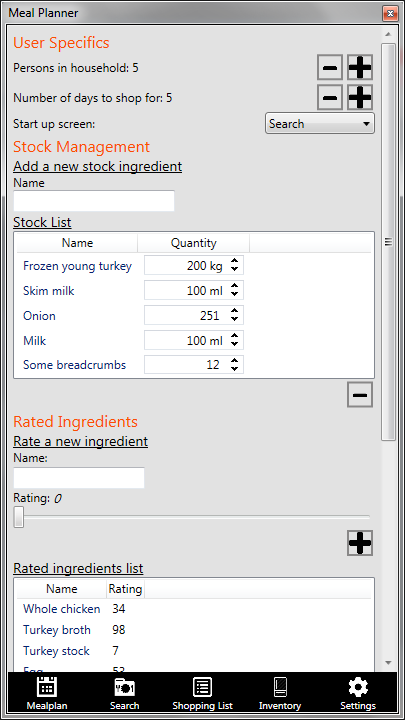
\includegraphics[width=.9\linewidth]{Grafik/SettingsPage}
  \captionof{figure}{Settings Page}
  \label{fig:SettnigsPage}
\end{minipage}%
\begin{minipage}{.33\textwidth}
  \centering
  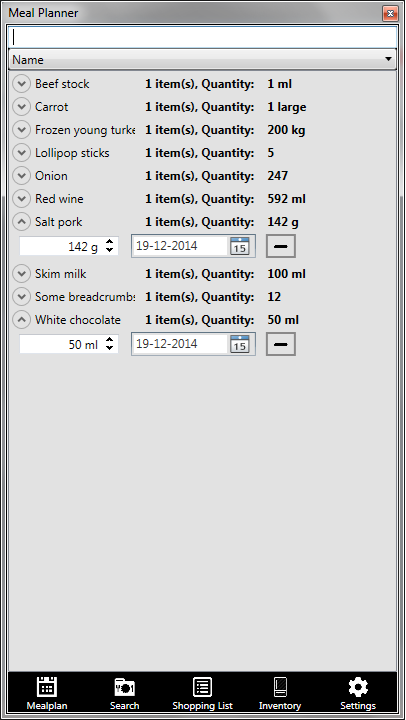
\includegraphics[width=.9\linewidth]{Grafik/InventoryPage}
  \captionof{figure}{Inventory Page}
  \label{fig:InventoryPage}
\end{minipage}%
\begin{minipage}{.33\textwidth}
  \centering
  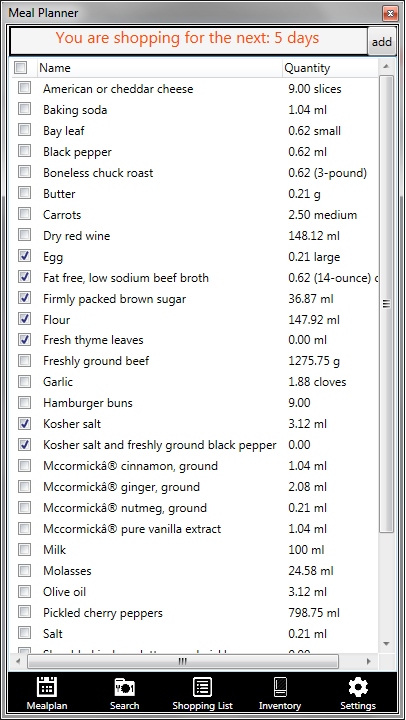
\includegraphics[width=.9\linewidth]{Grafik/ShoppingListPage}
  \captionof{figure}{Shopping List Page}
  \label{fig:ShoppingListPage}
\end{minipage}%
\end{figure}

\begin{figure}[H]
\centering
\begin{minipage}{.33\textwidth}
  \centering
  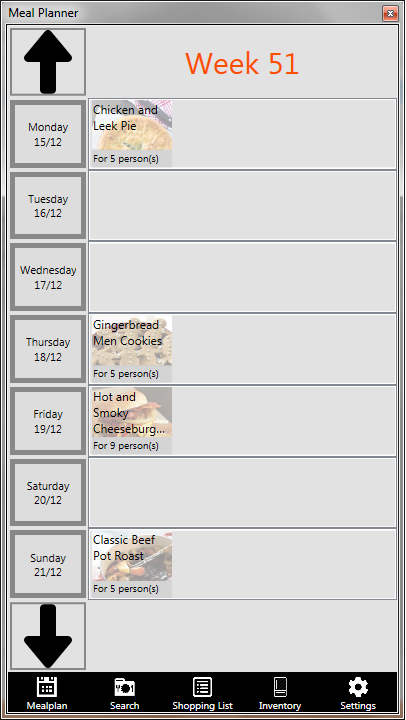
\includegraphics[width=.9\linewidth]{Grafik/MealPlanPage}
  \captionof{figure}{Meal Plan Page}
  \label{fig:MealPlanPage}
\end{minipage}%
\begin{minipage}{.33\textwidth}
  \centering
  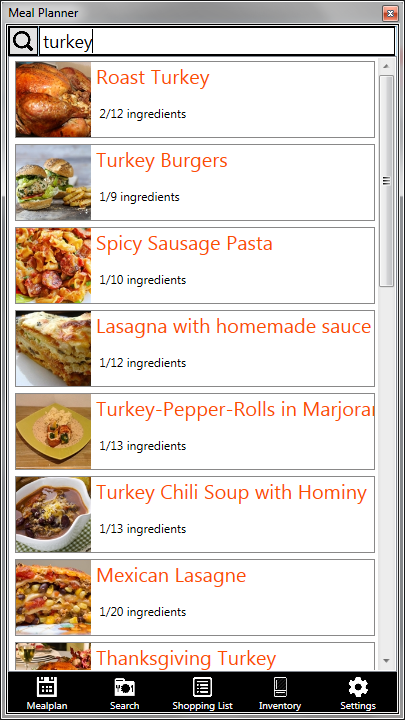
\includegraphics[width=.9\linewidth]{Grafik/SearchPage}
  \captionof{figure}{Search Page}
  \label{fig:SearchPage}
\end{minipage}%
\begin{minipage}{.33\textwidth}
  \centering
  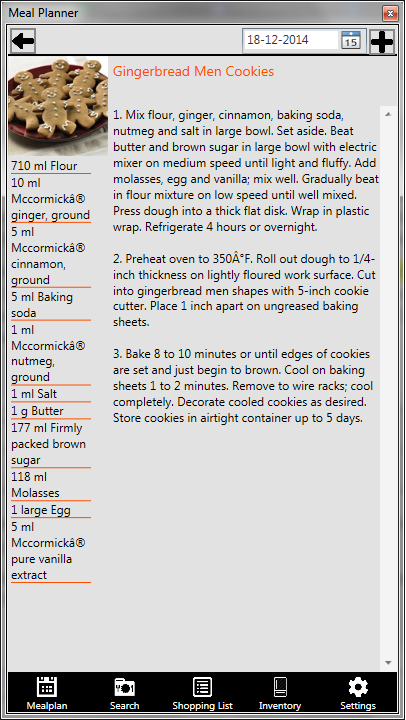
\includegraphics[width=.9\linewidth]{Grafik/RecipePage}
  \captionof{figure}{Recipe Page}
  \label{fig:RecipePage}
\end{minipage}%
\end{figure}

\subsection{Settings} \label{ss:settings}
The settings page, displayed on \cref{fig:SettnigsPage}, allows the user to specify different options for the program. The options are categorized as User Specifics, Stock Management, Rated Ingredients, Unwanted Ingredients and Diets.

Under the \textbf{User Specifics} category, you can change the how many persons that lives in the household, which is used as the default value for how many persons a meal should be scheduled for. You can also select how many days you want to shop ahead for, which means how many days in the future the shopping list takes into account. Finally you can select the default page, which the program shows when started.

The \textbf{Stock Management} category allows the user to add ingredients that they always want to have a specific quantity of. By typing the ingredient into a textbox with auto-completion as described in \cref{sec:AutoComplete} the user can select the ingredient. In the stock list the added stock ingredients are shown and the quantity can be changed by using numeric up-down control. The ingredient can be removed by selecting them and clicking the remove button symbolized with a minus (-) sign.

\textbf{Rated Ingredients} works the same way as \textbf{Stock Management} when adding an ingredient, but instead of setting a quantity, the user can give the ingredient a rating from 1-100 in order to prioritize the search, as described in \cref{ssc:graylist}. The user can also remove the ingredients from the rated ingredients list.

\textbf{Unwanted Ingredients} is similar to \textbf{Rated Ingredients} but the ingredients you add will instead be "blacklisted", as described in \cref{ssc:blacklist}, and thus completely remove recipes with these ingredients from the search.

\textbf{Diets} allows the user to choose a diet, which will make the search prioritize recipes that does not contain specific ingredients, so the user can keep a specific diet. The diets are pre set and can not be changed by the user.

\subsection{Inventory} \label{ss:inventory}
The inventory page, shown on \cref{fig:InventoryPage}, displays a list of the ingredients that the user have in the household. Initially the users sees all the ingredients from the inventory grouped by name, displaying the total quantity of each ingredient and how many individual ingredients there are. By expanding an ingredient with an expander control, the user can see the individual ingredients and change the quantity and expiration date.

In the top the users can add ingredients using the auto-complete control described in \cref{sec:AutoComplete}, which finds available ingredients from the database. The list is initially sorted by name, but can also be sorted by quantity or expiration date.

\subsection{Shopping List}
The shopping list page, displayed on \cref{fig:ShoppingListPage}, shows a list of ingredients that needs to be bought for the recipes in the meal plan within the shop-ahead period mentioned in \cref{ss:settings}. It displays ingredients and the quantity that is missing from the inventory, according to the meal plan and stock management settings. Each ingredient has a check-box so the user can add the selected ingredients directly to the inventory after shopping.

\subsection{Meal Plan}
The meal plan, illustrated on \cref{fig:MealPlanPage}, shows a week of scheduled meals, and allows the user to navigate to the previous and next week. The weekdays are listed as rows, with seven individual lists of meals belonging to the specific days. By clicking the meals the  user can navigate to the Recipe Page to see information about the recipe and/or update meal information.

\subsection{Search}
\Cref{fig:SearchPage} shows the Search page lists recipes sorted by multiple factors, first the Search is sorted by percentage of how many of the ingredients in the recipe the user has in the inventory, then the application sorts the list by the number of ingredients the user has partially in their inventory. Then the application sorts the search results by the rating of the ingredients in the recipe, then by how many times the ingredients in the recipe has been used in the past. Lastly the search results are sorted by the name of the recipe.
In the top it is possible to search for recipes by searching for the recipe name, or ingredients sorted by comma.

\subsection{Recipe Page}
On \cref{fig:RecipePage} the recipe page is shown. It shows information about a recipe or meal. By clicking a recipe in the search, you navigate to the recipe page which displays the title, image and description of the recipe as well as a list of ingredients. In the top you can add the recipe to the meal plan, and if it is already added you can update the date, or remove the recipe from the meal plan.
By clicking a meal on the meal plan the user is also taken to this page.

